\documentclass[11pt,a4paper]{article}

%
% $Id: userguide.tex 526 2007-10-31 08:57:09Z schnelle $
%

\usepackage[latin1]{inputenc}
\usepackage{graphics}
\usepackage{graphicx}
\usepackage{url}
\usepackage{listings}
\usepackage{xcolor}
\usepackage{jvoicexml}

\title{JVoiceXML Extension Guide}
\version{0.1.2}
\author{Dr. Dirk Schnelle-Walka}
\email{dirk.schnelle@jvoicexml.org}
\date{\today}

\begin{document}
\pagestyle{empty}
\lstset{language=Java,language=XML,
        backgroundcolor=\color{lightgray},
        basicstyle=\small,
        numbers=left,
        numberstyle=\tiny,
        stepnumber=5}

\maketitle

\pagestyle{headings}

\tableofcontents

\newpage

\begin{abstract}
This documents describes the API of JVoiceXML from the system integrator's point
of view. It provides information about how to hook your custom implementation
platform into the JVoiceXML voice browser.
\end{abstract}


\section{Introduction}
\label{sec:introduction}

JVoiceXML is a free VoiceXML~\cite{w3.org:voicexml} implementation written in 
the JAVA programming language. It offers a library for easy VoiceXML
document creation and a VoiceXML interpreter to process 
VoiceXML documents using JAVA standard APIs such as JSAPI~\cite{sun:jsapi} and
JTAPI~\cite{sun:jsapi}.

VoiceXML is hosted at SourceForge~\cite{sourceforge} as an open source project.
You find everything that is related to this project under
\url{http://sourceforge.net/projects/jvoicexml/}.
The work on the browser is still in progress and not all tags are
supported. You are invited to help us finishing the work to make this
project a success.

This document provides information on how to hook your custom implementation
platform into the JVoiceXML voice browser. It is assumed that readers are
familiar with the concepts of VoiceXML and Java programming.

This document refers to UNIX and Windows systems. JVoiceXML will work with 
any other operating systems that support Java 5, too.

Nobody is perfect, so you may find some errors or small things to correct.
Please let me know if you think you found something that should be written
differently or should be added.

\section{Copyright}
\label{sec:copyright}

JVoiceXML uses the GNU library general public license~\cite{gnu:lgpg}. 
You can find a copy in the file COPYING in the \$\{JVOICEXML\_HOME\}
directory. This means that you are allowed to use JVoiceXML
library in your commercial programs. If you make some nice
enhancements it would be great, if you could send us your
modifications so that we can make it available to the public.
If you make modifications to the existing code you must retain the concept of
making these modifications available for others. The best way to to this is to
send us your modifications.

While JVoiceXML is an open source project and you have a short
description in your hands you might be looking for help with implementing your
implementation platform or with your JVoiceXML project. Have a look at our
contact page and ask for consulting services.

\subsection{Lesser GNU Public License}

JVoiceXML is free software; you can redistribute it and/or
modify it under the terms of the GNU Library General Public
License as published by the Free Software Foundation; either
version 2 of the License, or (at your option) any later version.

JVoiceXML is distributed in the hope that it will be useful,
but WITHOUT ANY WARRANTY; without even the implied warranty of
MERCHANTABILITY or FITNESS FOR A PARTICULAR PURPOSE. See the GNU
Library General Public License for more details.

You should have received a copy of the GNU Library General Public
License along with this library; if not, write to the Free
Foundation, Inc., 59 Temple Place, Suite 330, Boston, MA  02111-1307  USA

\section{Architectural Overview}
\label{sec:arch-overv}

Before going into detail the general architecture and concepts are presented.
The basic architecture is shown in figure~\ref{fig:main-components}.
\begin{figure}
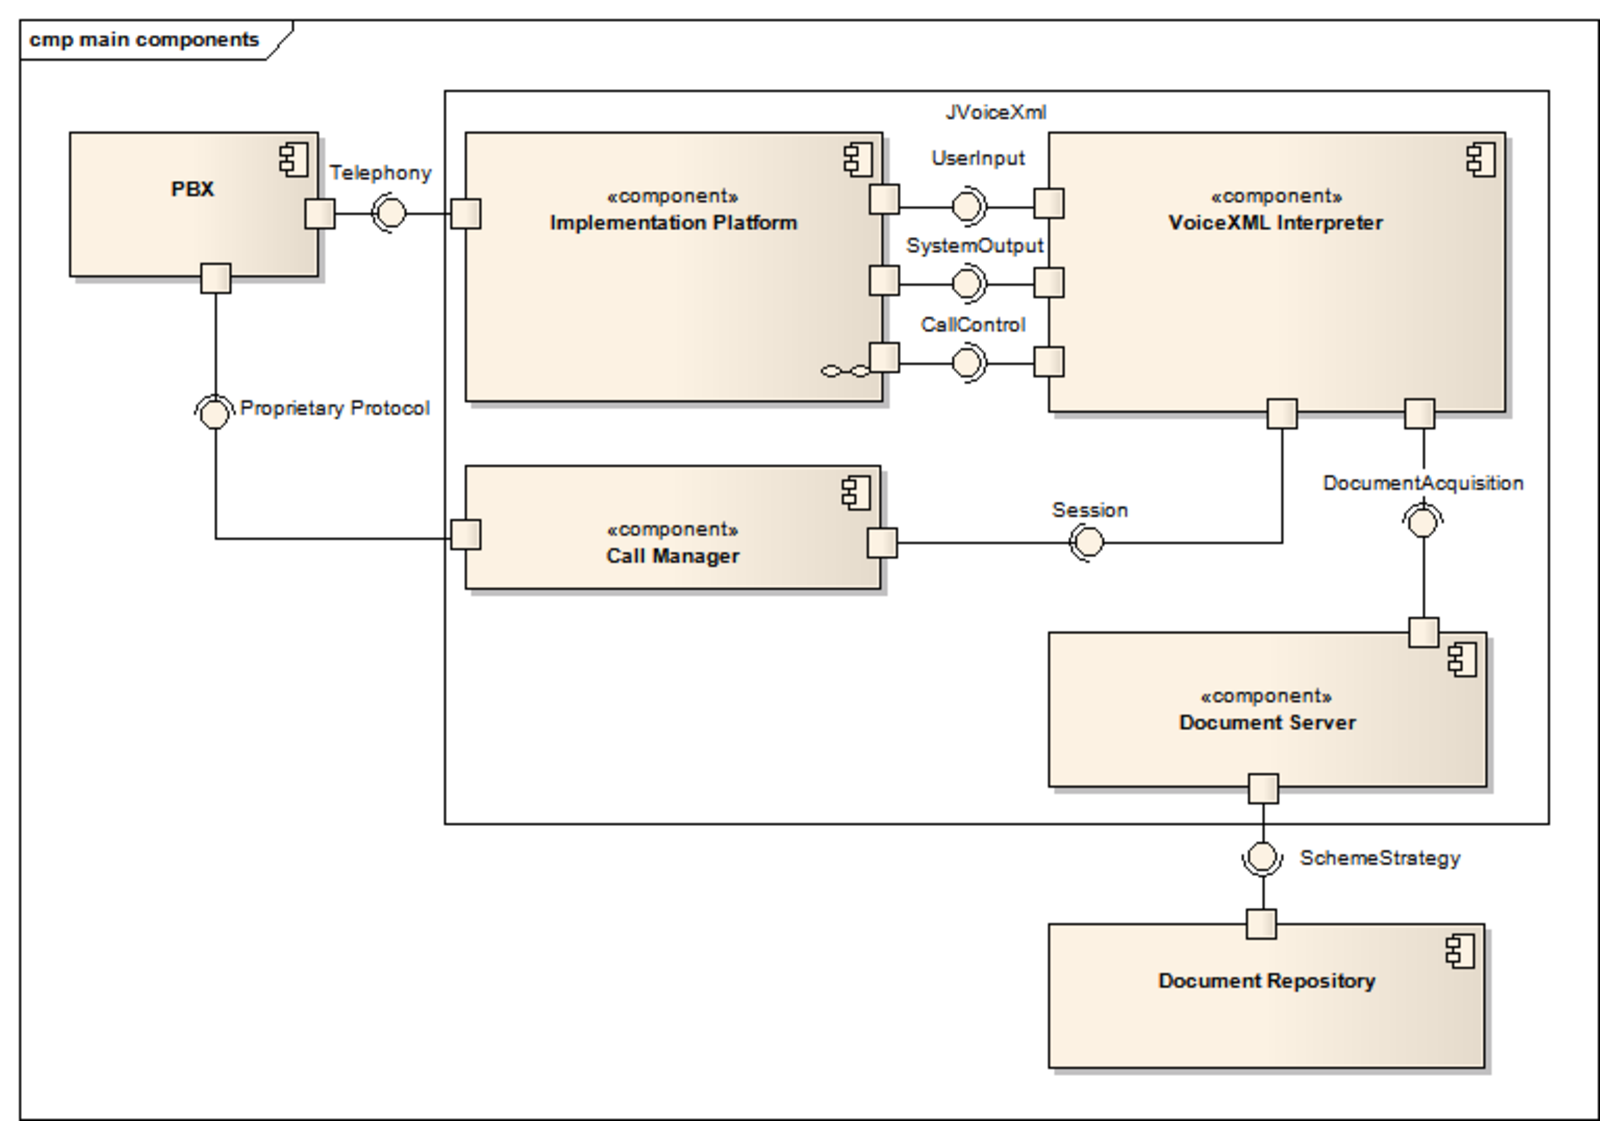
\includegraphics[width=\linewidth]{cd-main-components}
\caption{Basic architecture of JVoiceXML}
\label{fig:main-components}
\end{figure}
The point of interest is the \emph{Implemtation Platform}.
Figure~\ref{fig:implementationplatform} shows the composite parts of that
component.
\begin{figure}
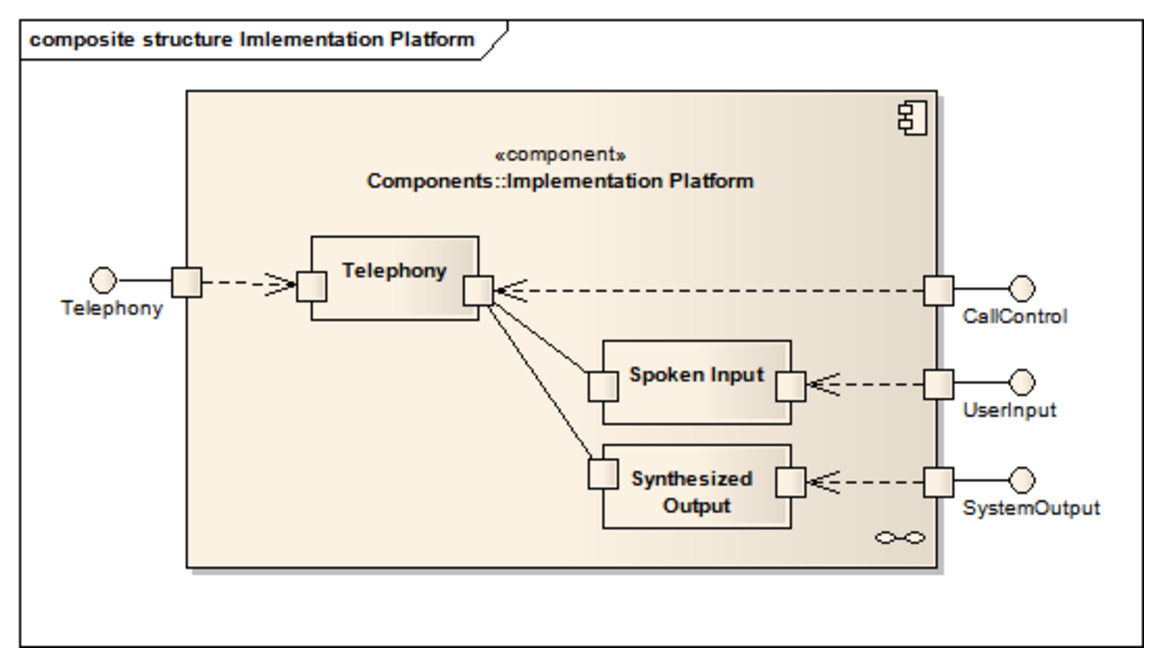
\includegraphics[width=\linewidth]{csd-implementation-platform}
\caption{Composite parts of the implementation platform}
\label{fig:implementationplatform}
\end{figure}

\section{Steps to your own implementation platform}

In this section a first cookbook on how to create your own imlementation
platform is presented. Currently there is only some basic content to help you
getting started.


\subsection{RemoteClient}

A remote client is a data container that holds all the information that is
needed to connect the server side resources. Therefore you have to implement
the \lstinline[language=Java]{org.jvoicexml.RemoteClient} interface. This
container is used to transfer all the information that is needed to connect to
your client application from the JVoiceXML resources to the JVoiceXML server.

The identification of remote clients is based on strings. Choose a unique name
for each of your resource types. It is legal to have the same name for all your
types.

The \lstinline[language=Java]{RemoteClient} object is passed to the external
resources once they are obtained from the pool, see
figure~\ref{fig:get-external-resource-from-pool}. The resources are identified
using the custom string. By calling the
\lstinline[language=Java]{connect(RemoteClient)} method the
\lstinline[language=Java]{RemoteClient} object is delivered to the resource and
can be used to grab the connection information.
\begin{figure}[htp]
\begin{center}
  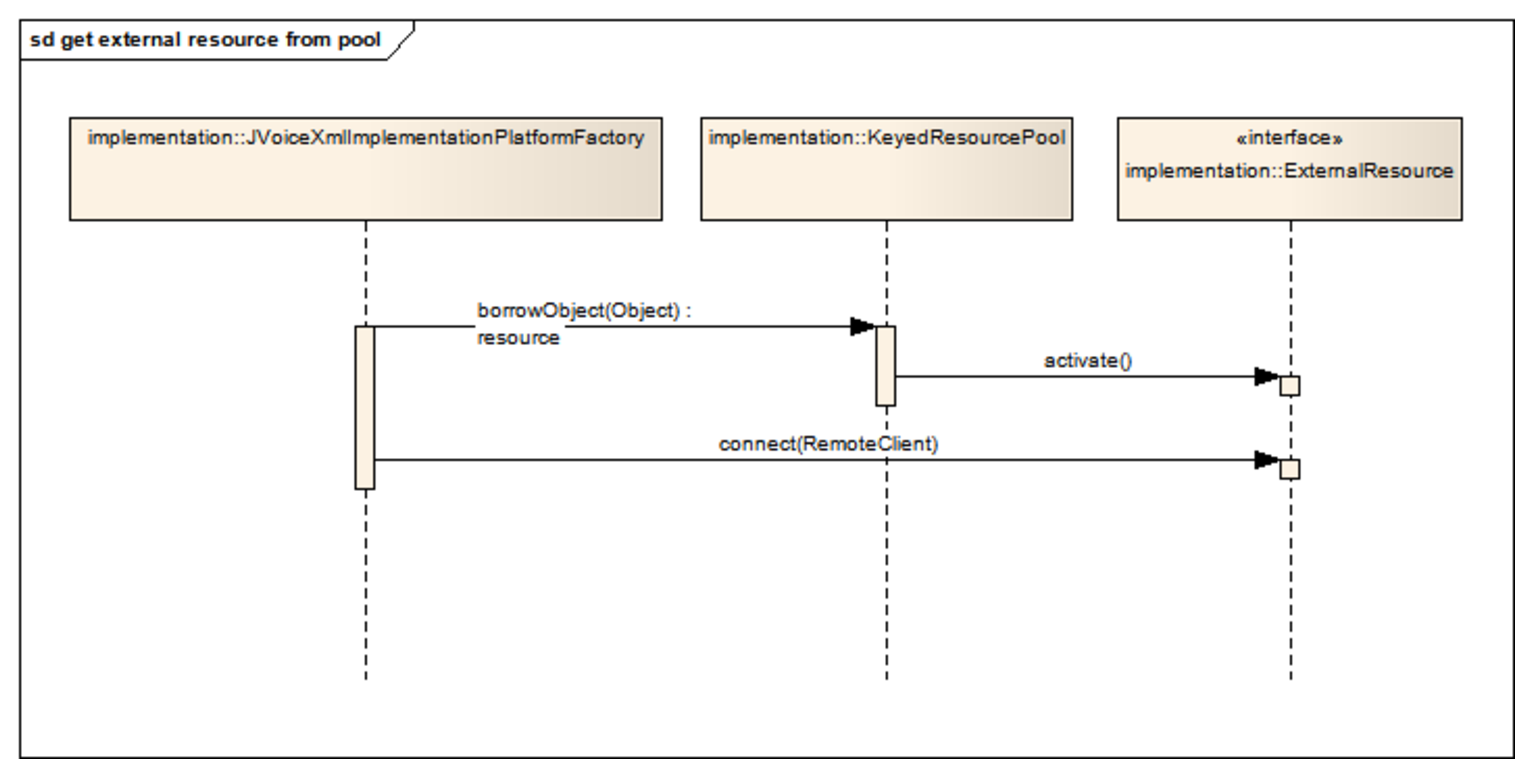
\includegraphics[width=\linewidth]{sd-get-external-resource-from-pool}
  \caption{Get external resource from pool}
  \label{fig:get-external-resource-from-pool}
\end{center}
\end{figure}

Note that \lstinline[language=Java]{RemoteClient} implementations must also
implement \lstinline[language=Java]{java.io.Serializable} to stream the object
from your client to the JVoiceXML voice browser.

\subsection{Resources}

The first step is to write your own implementations of the resources:
\begin{itemize}
  \item \lstinline[language=Java]{org.jvoicexml.implementation.SpokenInput}
  \item
  \lstinline[language=Java]{org.jvoicexml.implementation.SynthesizedOutput}
  \item \lstinline[language=Java]{org.jvoicexml.implementation.Telephony}
\end{itemize}

Before you start you have to understand the lifecyle of a resource which is
shown in figure~\ref{fig:external-resource-lifecycle}.
\begin{figure}[htp]
\begin{center}
  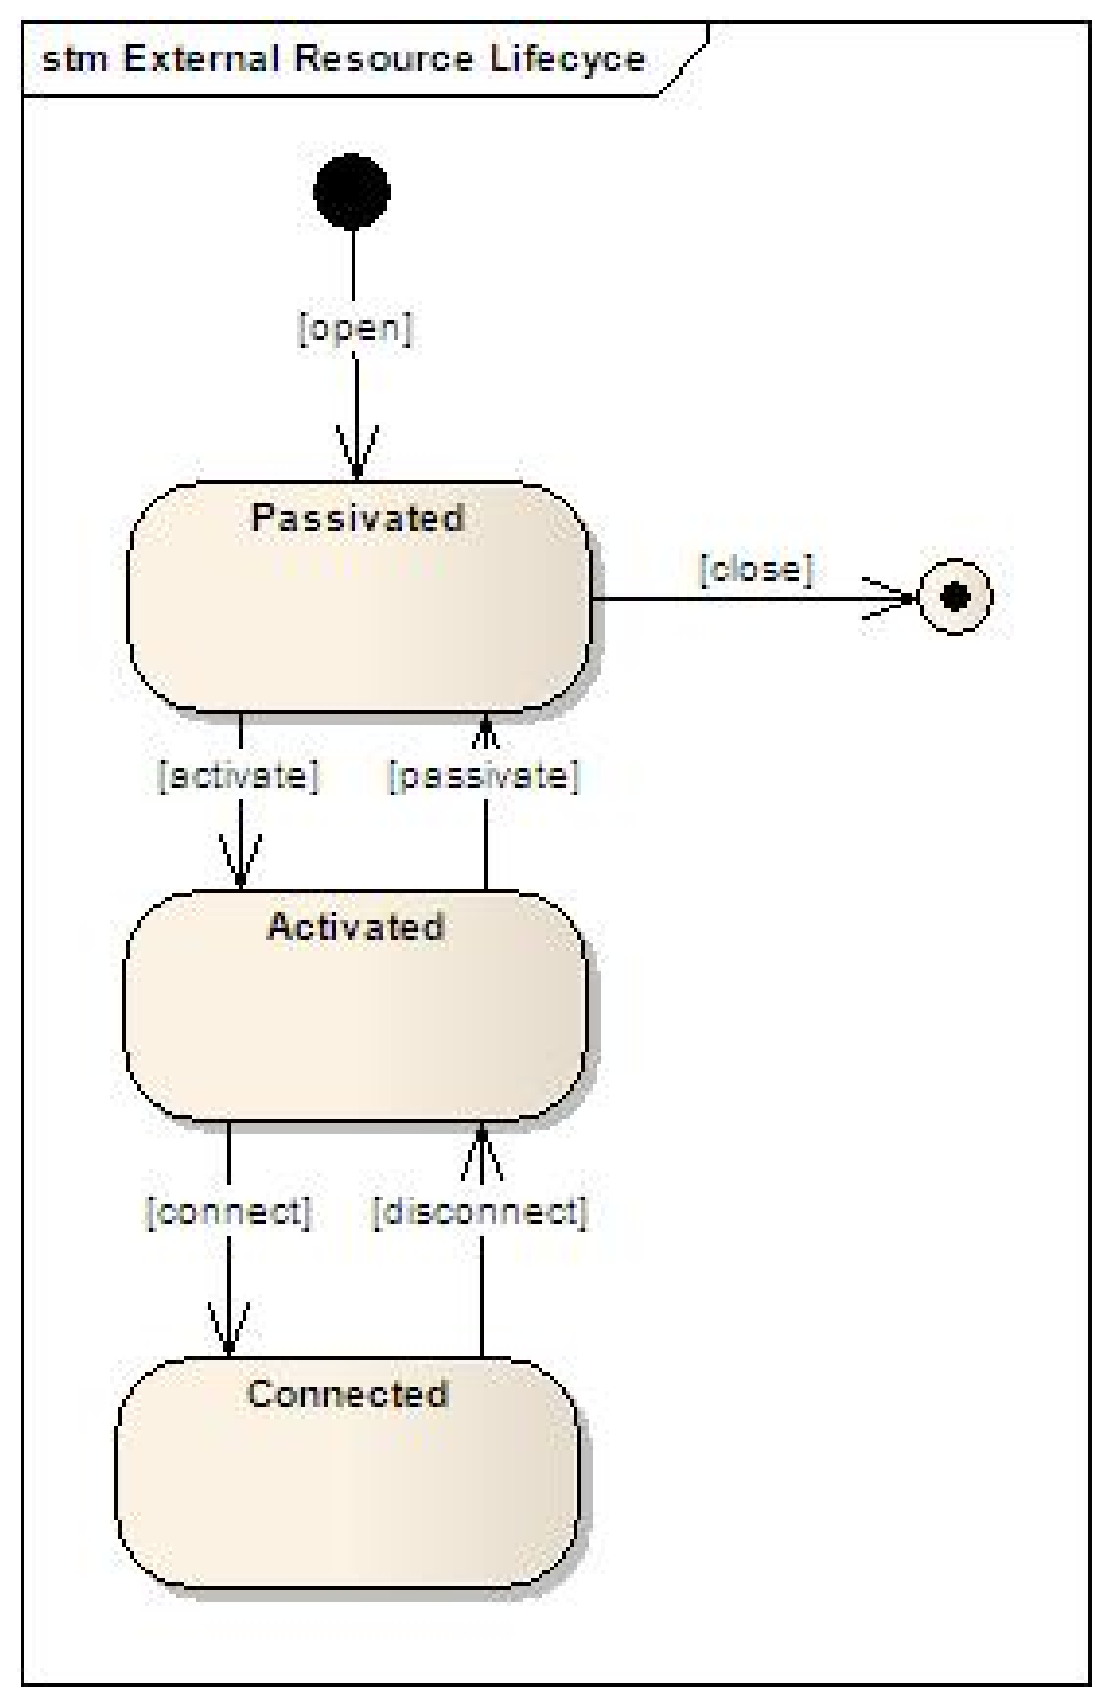
\includegraphics[width=0.4\linewidth]{stm-external-resource-lifecycle}
  \caption{External resource lifecycle}
  \label{fig:external-resource-lifecycle}
\end{center}
\end{figure}
Each transisition is reflected by a corresponding method in the interface
\lstinline[language=Java]{org.jvoicexml.implementation.ExternalResource}
that has to be implemented, see figure~\ref{fig:external-resource}.
\begin{figure}[htp]
\begin{center}
  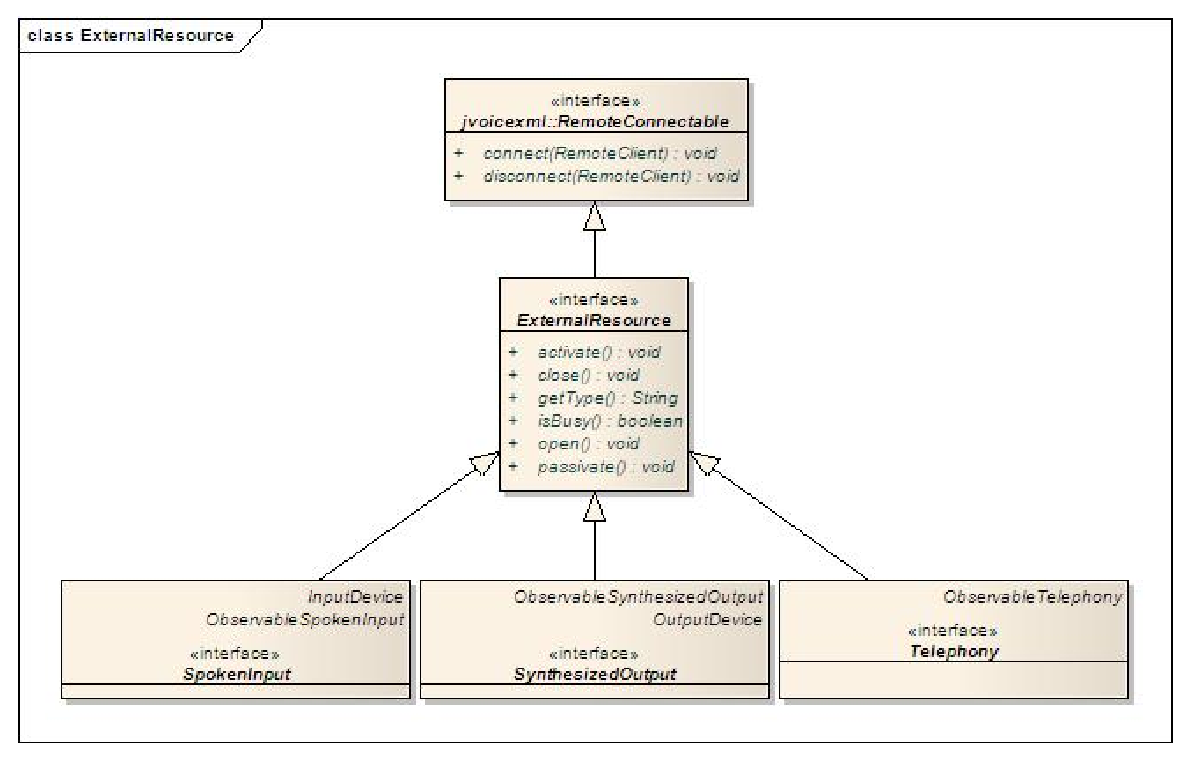
\includegraphics[width=\linewidth]{class-external-resource}
  \caption{External resource inheritance}
  \label{fig:external-resource}
\end{center}
\end{figure}

Your \lstinline[language=Java]{SynthesizedOutput} implementation should maintain
a queue of speakables that should be sent to your client.

Your \lstinline[language=Java]{Telephony} implementation should be able to
conect to your client. It takes the speakables from your Your
\lstinline[language=Java]{SynthesizedOutput} Sending it to your client and also
retrieve inputs from the client. These are forwarded to your 
\lstinline[language=Java]{SpokenInput} implementation. The latter one is
responsible to notify the JVoiceXML voice browser about incoming speech events.

Figure~\ref{fig:play} shows how the voice browser addresses the resources to
queue a \lstinline[language=Java]{Speakable}.
\begin{figure}[htp]
\begin{center}
  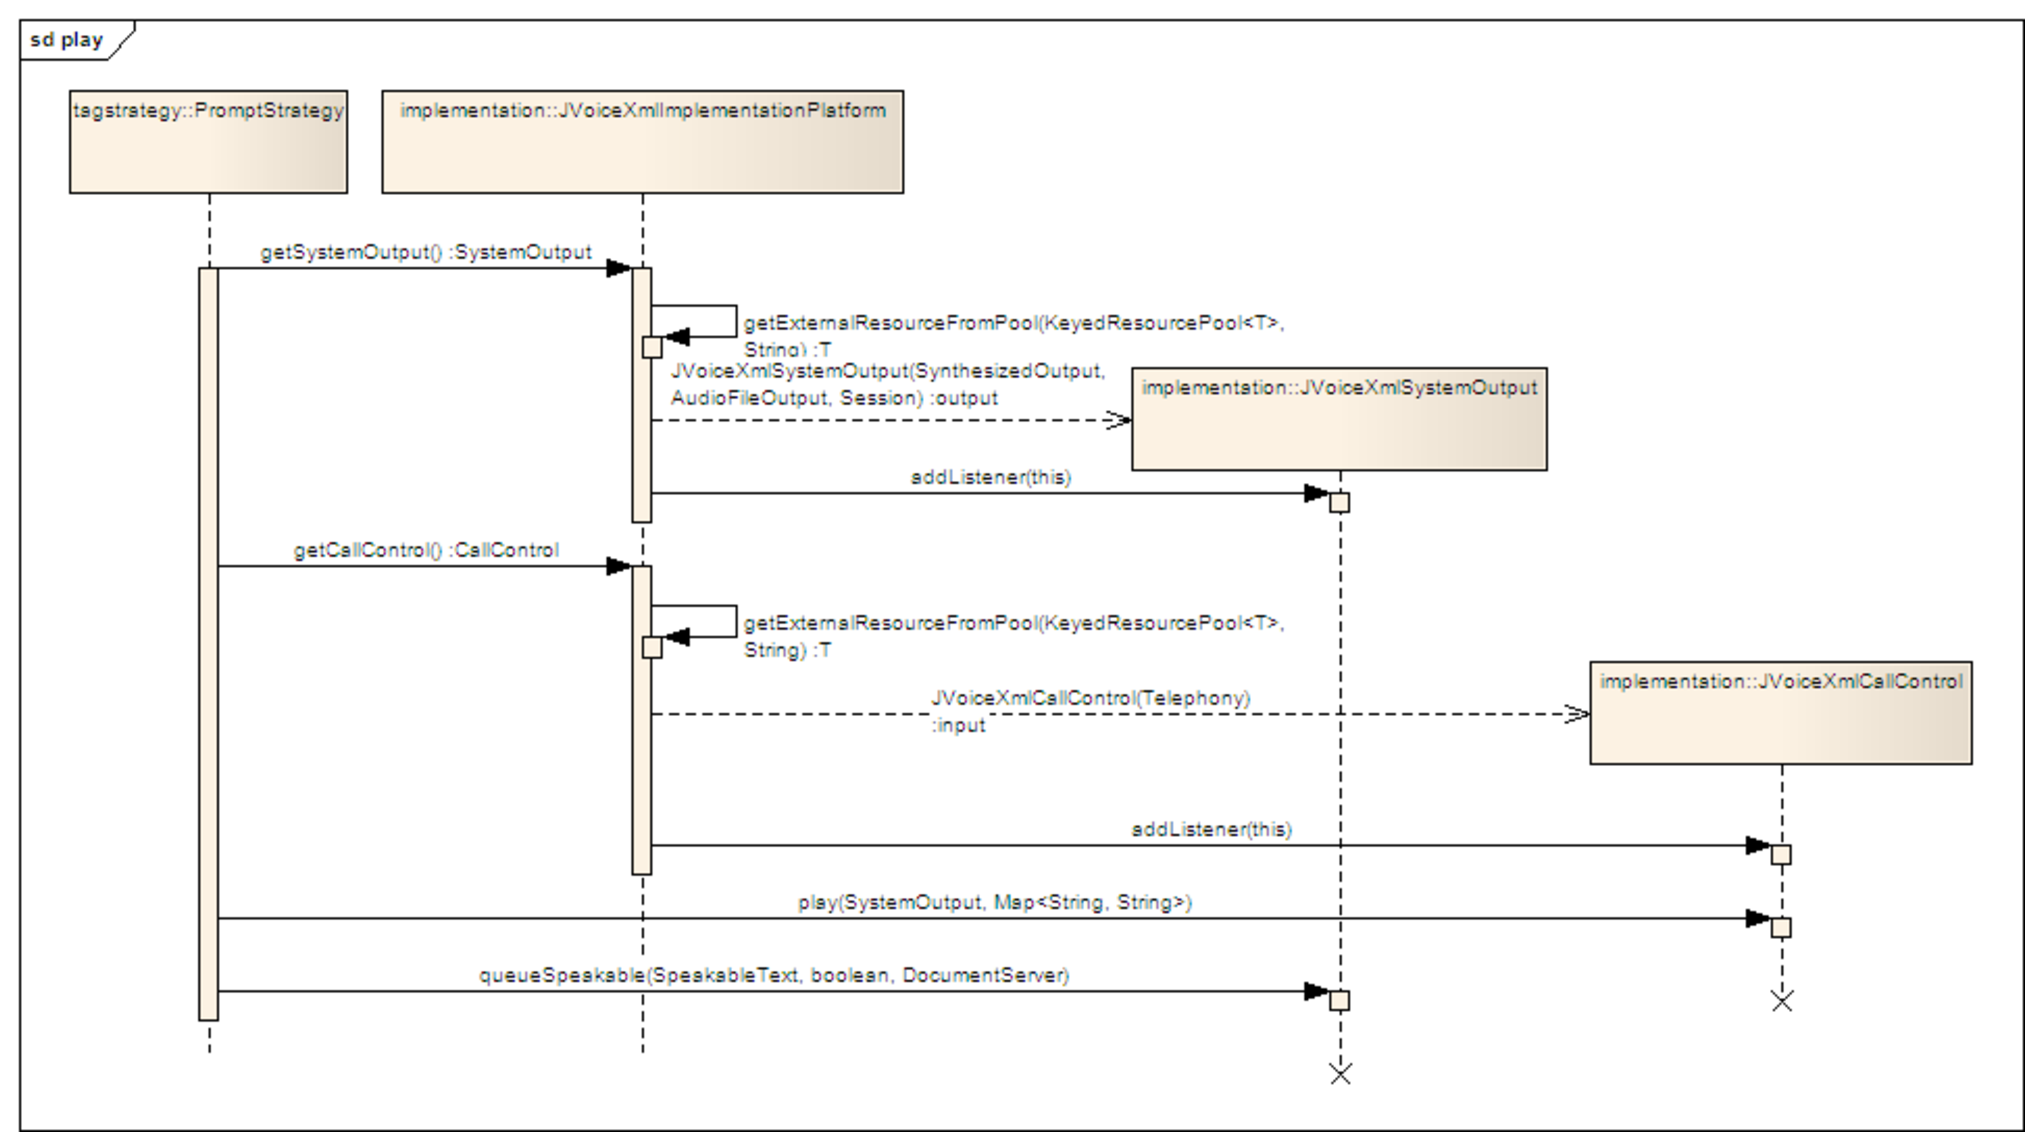
\includegraphics[width=\linewidth]{sd-play}
  \caption{Prompt queuing of the PromptStrategy}
  \label{fig:play}
\end{center}
\end{figure}
JVoiceXML does not make any assumptions how the implementation resources
transfer the \lstinline[language=Java]{Speakable}s from the
\lstinline[language=Java]{SynthesizedOutput} implementation to the
\lstinline[language=Java]{Telephony} implementation. That's why the
\lstinline[language=Java]{SynthesizedOutput} is passed to the
\lstinline[language=Java]{Telephony} implementation as the argument in a
\lstinline[language=Java]{play} call.

The resources communicate with the JVoiceXML voice browser using a
notification mechanism. Hence it is important that the custom resource classes also implement
the corresponding notification interfaces.

\begin{itemize}
  \item the \lstinline[language=Java]{SpokenInput} resource must also implement
  \\
  \lstinline[language=Java]{org.jvoicexml.implementation.ObservableSpokenInput}
  \item the \lstinline[language=Java]{SynthesizedOutput} resource must also
  implement \\
  \lstinline[language=Java]{org.jvoicexml.implementation.ObservableSynthesizedOutput}
  \item the \lstinline[language=Java]{Telephony} resource must also implement \\
  \lstinline[language=Java]{org.jvoicexml.implementation.ObservableTelephony}
\end{itemize}

\subsection{Resource factories}

The implementation platform retrieves the resources via a
\lstinline[language=Java]{org.jvoicexml.implementation.ResourceFactory}.
Implement a factory for each of your resources.

Return the type that you defined in your
\lstinline[language=Java]{RemoteClient} implementation.

\subsection{JVoiceXML configuration}

JVoiceXML retrieves the resource factories via dependency injection from
configuration files that are located in
\lstinline{$JVOICEXML_HOME/config}. Implementation platform configuration files
must use the \lstinline{jvxml-implementation-version.xsd} schema file.
An example is shown below:

\begin{lstlisting}[language=XML]
<?xml version="1.0" encoding="UTF-8"?>
<implementation xmlns:beans=
      "http://www.springframework.org/schema/beans"
  xmlns:xsi="http://www.w3.org/2001/XMLSchema-instance"
  xsi:noNamespaceSchemaLocation=
      "jvxml-implementation-0-7.xsd">
  <repository>text</repository>
  <classpath>dist/jvxml-text.jar</classpath>
  <classpath>dist/jvxml-client-text.jar</classpath>
  <beans:bean class=
    "org.jvoicexml.implementation.text.TextPlatformFactory">
    <beans:property name="instances" value="8" />
  </beans:bean>
</implementation>
\end{lstlisting}

All tags prefixed with \lstinline{beans} are inherited by the SPRING. Custom
tags are \lstinline{classpath} and \lstinline{repository}. The
\lstinline{classpath} tag allows to add your custom jar files and all third
party jar files that are needed by your implementation platform. By default
JVoiceXML uses an own class loader for these jar files. This way it is possible
to have different versions of the same jar in different implementation
platforms at the same time. The \lstinline{repository} tag allows you to
uniquely identify this class loader repository. Sometimes it is necessary to
share the same repository e.g. with a \lstinline[language=Java]{CallManager}.
Note that Java considers two classes loaded from different class loaders as
different classes.

\bibliography{extensionguide}
\bibliographystyle{plain}

\end{document}
